% =====================================================================
\documentclass[a4paper,11pt]{article}
% Minimal standalone preamble for the verification supplement.
\usepackage[T1]{fontenc}
\usepackage{lmodern}
\usepackage{amsmath,amssymb,amsthm,mathtools}
\usepackage{booktabs,longtable,supertabular,array}
\usepackage{enumitem}
\usepackage{etoolbox}
\usepackage{needspace}
\usepackage{tikz}
\usetikzlibrary{positioning,arrows.meta}
\usepackage[font=small,labelfont=bf,skip=4pt]{caption}
\usepackage[hidelinks]{hyperref}
\usepackage{url}
\usepackage{xcolor}
\usepackage{microtype}
\usepackage[htt]{hyphenat}

\newcolumntype{P}[1]{>{\raggedright\arraybackslash}p{#1}}
\newcommand{\TableStart}{\needspace{8\baselineskip}}
\newcommand{\TableHeader}{}
\newcommand{\TableRowRule}{\specialrule{0.25pt}{0.18ex}{0.18ex}}
\setlength{\tabcolsep}{4pt}
\setlength{\extrarowheight}{0.6pt}
\renewcommand{\arraystretch}{1.08}
\setlength{\emergencystretch}{2em}
\raggedbottom
\sloppy
\allowdisplaybreaks
\newtheorem{theorem}{Theorem}[section]
\newtheorem{lemma}[theorem]{Lemma}
\newtheorem{proposition}[theorem]{Proposition}
\newtheorem{corollary}[theorem]{Corollary}
\newtheorem{definition}[theorem]{Definition}
\newtheorem{construction}[theorem]{Construction}
\newtheorem{numerical}[theorem]{Numerical result}
\newtheorem{nogo}[theorem]{No-go result}
% Zenodo DOI of the archived release; replaced once the DOI is minted.
\providecommand{\ZenodoDOI}{10.5281/zenodo.XXXXXXX}
% Long and split tables: centred, and separated from the surrounding text.
\usepackage{etoolbox}
\setlength{\LTpre}{\bigskipamount}
\setlength{\LTpost}{\bigskipamount}
\setlength{\LTleft}{0pt plus 0.5\textwidth}
\setlength{\LTright}{0pt plus 0.5\textwidth}
\BeforeBeginEnvironment{supertabular}{\par\addvspace{\bigskipamount}}
\AfterEndEnvironment{supertabular}{\par\addvspace{\bigskipamount}}

\title{Verification and Reproducibility Supplement}
\author{Youngik (Tom) Lee}
\begin{document}
\raggedbottom
\sloppy
\maketitle
\section*{Scope}
This supplement contains the Lean correspondence, the calculation index and
the numerical provenance of the main paper. It supports the arguments of the
paper and does not add to its logical model or change any of its conclusions.
% =====================================================================
\section{Formal verification and Lean correspondence}\label{app:lean}
The formal counterpart is checked against a Lean~4 project using mathlib. It is
kept in the public repository \url{https://github.com/s6ygleee/torus-node-lean4}
and intended for archival on Zenodo (DOI: \ZenodoDOI)~\cite{TorusLean2026}. The
Yang--Mills follow-up paper has its own formalisation, released with that paper.
The project verifies explicitly listed
subclaims; they are not a machine-checked proof of every statement in this
paper.

\begin{figure}[!ht]
\centering
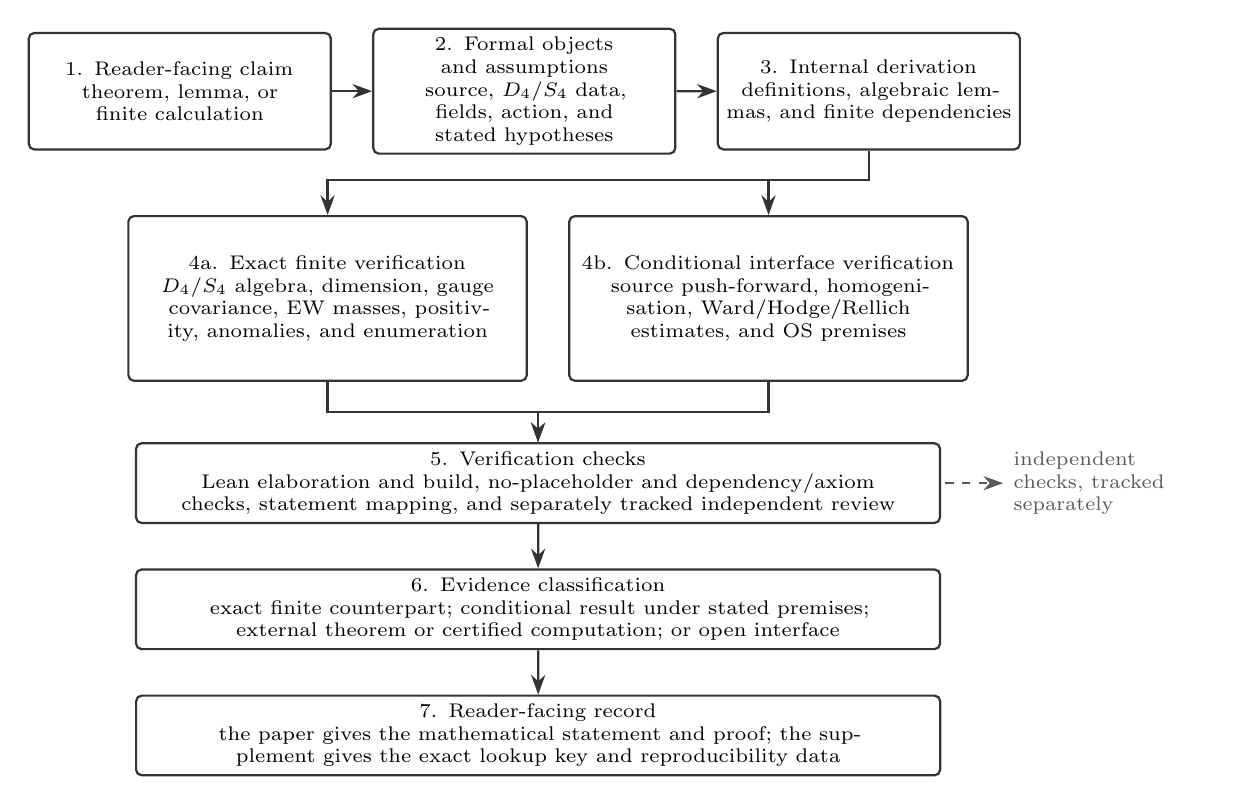
\begin{tikzpicture}[scale=1.02,transform shape,
  node distance=0.55cm and 0.50cm,
  leanstep/.style={draw=black!80,thick,rounded corners=2pt,align=center,
    text width=3.55cm,minimum height=1.45cm,inner sep=3pt,font=\scriptsize},
  leanbranch/.style={draw=black!80,thick,rounded corners=2pt,align=center,
    text width=4.75cm,minimum height=2.05cm,inner sep=3pt,font=\scriptsize},
  leanwide/.style={draw=black!80,thick,rounded corners=2pt,align=center,
    text width=9.80cm,minimum height=0.80cm,inner sep=3pt,font=\scriptsize},
  leanarrow/.style={-{Stealth[length=2.5mm,width=1.8mm]},thick,black!80},
  leandash/.style={-{Stealth[length=2.5mm,width=1.8mm]},thick,dashed,black!65}
]
\node[leanstep] (statement) {1. Reader-facing claim\\theorem, lemma, or finite calculation};
\node[leanstep,right=of statement] (objects) {2. Formal objects and assumptions\\source, $D_4/S_4$ data, fields, action, and stated hypotheses};
\node[leanstep,right=of objects] (derivation) {3. Internal derivation\\definitions, algebraic lemmas, and finite dependencies};
\draw[leanarrow] (statement)--(objects);
\draw[leanarrow] (objects)--(derivation);

\node[leanbranch,below=0.75cm of objects,xshift=-2.45cm] (finite) {4a. Exact finite verification\\$D_4/S_4$ algebra, dimension, gauge covariance, EW masses, positivity, anomalies, and enumeration};
\node[leanbranch,right=0.50cm of finite] (conditional) {4b. Conditional interface verification\\source push-forward, homogenisation, Ward/Hodge/Rellich estimates, and OS premises};
\draw[leanarrow] (derivation.south) -- ++(0,-0.37cm) -| (finite.north);
\draw[leanarrow] (derivation.south) -- ++(0,-0.37cm) -| (conditional.north);

\node[leanwide,below=0.75cm of finite,xshift=2.62cm] (checks) {5. Verification checks\\Lean elaboration and build, no-placeholder and dependency/axiom checks, statement mapping, and separately tracked independent review};
\draw[leanarrow] (finite.south) -- ++(0,-0.37cm) -| (checks.north);
\draw[leanarrow] (conditional.south) -- ++(0,-0.37cm) -| (checks.north);

\node[leanwide,below=of checks] (class) {6. Evidence classification\\exact finite counterpart; conditional result under stated premises; external theorem or certified computation; or open interface};
\draw[leanarrow] (checks)--(class);
\node[leanwide,below=of class] (record) {7. Reader-facing record\\the paper gives the mathematical statement and proof; the supplement gives the exact lookup key and reproducibility data};
\draw[leanarrow] (class)--(record);
\draw[leandash] (checks.east) ++(0.05cm,0) -- ++(0.72cm,0) node[right,align=left,text width=2.3cm,font=\scriptsize] {independent checks, tracked separately};
\end{tikzpicture}
\caption{Categorised verification path.  The formal work proceeds from a reader-facing mathematical claim to the finite objects and assumptions on which it depends, then to internal derivations.  Exact finite statements and conditional interface statements are kept as separate branches before the machine checks and the final evidence classification.  A successful build certifies only the listed formal statements and their dependencies; it does not convert an external theorem or an open source--continuum interface into an internally proved result.}
\label{fig:lean-verification-flow}
\end{figure}

The formalisation has a conditional scope: it covers the listed Lean statements
and their dependencies, but it does not formalise every assertion in the paper.
Two independent machine checks support those statements.  The first is the Lean
kernel itself, run during the build.  The second replays the compiled
declarations outside Lean: every project module is exported with
\texttt{lean4export} and re-checked by the independent type checker
\mbox{nanoda}, in bounded batches of modules together with all of their
transitive dependencies.  All 84 project modules were checked in eleven batches; nanoda reported no
type-checking errors.  Neither check decides whether a Lean
statement says the same thing as the surrounding prose; that correspondence is
reviewed separately and still requires human approval.

The formal record has the following content.
\begin{itemize}[leftmargin=*]
\item The Lean~4.32.1 project builds without errors, and the placeholder,
  dependency, axiom and statement-mapping checks pass for all 296 inventory
  declarations.  The inventory lists formal statements; it is not the count of
  results in the paper.
\item The main paper contains 112 theorem-like environments: 4 explicit
  hypotheses and 108 other environments, namely 10 definitions and 98 results,
  each result with a local proof.  Of these 108 environments, 12 are formalised
  exactly, 54 through a finite or conditional core, and 38 through formalised
  lemmas or cited external results; the four results on confinement under
  the window hypothesis in the Yang--Mills interface section have no Lean
  counterpart, and the four hypotheses are not formalised.
  The classification is complete, so every stated result has a recorded formal
  status.
\item The only axioms reported for the audited declarations are the standard
  Lean axioms \texttt{propext}, \texttt{Classical.choice} and
  \texttt{Quot.sound}.  An external mathematical theorem used in a proof is
  therefore an explicit hypothesis of the corresponding Lean statement, not a
  hidden axiom.
\item The Yang--Mills follow-up is a separate project with its own build and
  checks; it is not part of the present verification count.
\end{itemize}
The formalisation therefore checks the listed formal statements and their
machine dependencies.  The source-to-continuum bridge and the remaining
certified numerical-to-analytic interfaces are open obligations rather than
hidden assumptions.

Each row begins with a reader-facing mathematical statement.  The second
column gives the exact machine lookup key used by the corresponding Lean
checker.  Namespaces and qualified identifiers such as
\texttt{TorusModel.FiniteCompletion.*} are repository-local implementation names, not
mathematical notation or physical model names.  They are retained verbatim
only so that the formal correspondence can be reproduced; the first column
is the authoritative description for readers of the theory.

\clearpage
{\scriptsize\TableStart
\tablecaption{Correspondence between reader-facing statements and formal counterparts.}
\tablehead{\toprule\TableHeader Reader-facing statement & Formal counterpart (exact lookup key)\\\midrule}
\begin{supertabular}{P{0.30\textwidth}@{\hspace{0.35em}} P{0.64\textwidth}}
\multicolumn{2}{l}{\emph{Part I} (namespace \texttt{TorusModel})}\\
Lemma (D4 quartic and layers) & \texttt{D4.root\_card}, \texttt{D4.weighted\_root\_sum\_Q4}, \texttt{D4.cosine\_series\_eq}, \texttt{D4.quartic\_formula}, \texttt{D4.d4\_cosine\_quartic\_coefficient}, \texttt{TorusModel.D4\_quartic\_isotropic}, \texttt{TorusModel.D4\_layers\_core}\\
\TableRowRule
Definition/proposition (wave law) & \texttt{TorusModel.wave\_law}, \texttt{TorusModel.wave\_law\_area\_scaling}\\
\TableRowRule
Spacetime coordinate dimension core & \texttt{TorusModel.dim\_four}\\
\TableRowRule
Finite Gaussian electroweak lower-bound statement & \texttt{TorusModel.EWC\_gaussian}\\
\TableRowRule
Finite history-renormalisation contraction & \texttt{TorusModel.history\_RG\_contraction}\\
\TableRowRule
Finite physical-time lift & \texttt{TorusModel.lift\_S2}\\
\TableRowRule
Finite common-light-cone statement & \texttt{TorusModel.common\_lightcone}\\
\TableRowRule
Poisson--Lorentz expectation statement & \texttt{TorusModel.poisson\_lorentz}\\
\TableRowRule
Annealed reflection-positivity statement & \texttt{TorusModel.annealed\_RP}\\
\TableRowRule
Conditional high-density homogenisation certificate & \texttt{TorusModel.high\_density\_homogenisation\_conditional}; algebraic ingredients \texttt{TorusModel.vertex\_addition}, \texttt{TorusModel.Q3\_lower}\\
\TableRowRule
Finite reflection-positivity Gram inequality & \texttt{TorusModel.FiniteCompletion.gram\_quadratic\_nonneg}\\
\TableRowRule
Finite electroweak bath and local Gaussian realisation & {\scriptsize \texttt{TorusModel.FiniteCompletion.bath\_memory\_quadratic\_nonneg}, \texttt{TorusModel.FiniteCompletion.bath\_memory\_eq\_gram}}\\
\TableRowRule
Finite plaquette gauge covariance & {\scriptsize \texttt{TorusModel.FiniteCompletion.plaquette\_gauge\_transform}}\\
\TableRowRule
Tree-level electroweak $\rho$ relation & \texttt{TorusModel.EW1.mass\_ratio\_cosTheta}\\
\TableRowRule
Theorem 6.13 (Chirality, charges and anomalies) & \texttt{three\_generations}, \texttt{anomaly\_traces}, \texttt{anomaly\_traces\_three\_generations}, \texttt{charge\_quantization}, \texttt{bifundamental\_hypercharge}, \texttt{green\_schwarz\_cancellation}\\
\TableRowRule
Lemma 8.4 (Gauss-law lemma) & \texttt{GL.GL\_core}, \texttt{GL.GL\_massless}, \texttt{GL.not\_summable}, \texttt{GL.psd\_lower\_bound\_kernel}, \texttt{GL.gauss\_range\_subset\_kernel}, \texttt{GL.continuous\_fourier}, \texttt{GL.summable\_fourierTerm}\\
\TableRowRule
Lemma 8.9 (Rank-one defect) & \texttt{HWD.rank\_one\_energy\_update}\\
\TableRowRule
Lemma 8.12 (Holonomies of holes decouple) & \texttt{HC.weight\_invariant}, \texttt{HC.curvature\_observable\_indep}, \texttt{HC.rational\_kernel\_subtorus\_closed}, \texttt{HC.rational\_kernel\_subtorus\_in\_kernel}, \texttt{HC.integer\_torus\_image\_closed}, \texttt{HC.compact\_torus\_image\_closed}, \texttt{HC.ker\_closed\_in\_finite\_dimension}, \texttt{HC.integer\_torus\_map\_comp}, \texttt{HC.integer\_torus\_map\_comp\_eq\_zero}, \texttt{HC.product\_measure\_expectation\_factor}, \texttt{HC.conditional\_probability\_eq\_addHaar}\\
\TableRowRule
Theorem 8.14 (Isotropy) & {\scriptsize \texttt{TorusModel.Q2.exists\_separating}, \texttt{TorusModel.Q2.offdiag\_zero}, \texttt{TorusModel.Q2.equal\_diagonal\_of\_transitive}, \texttt{TorusModel.Q2.scalar\_of\_invariant}, \texttt{TorusModel.Q2.pairAction\_transitive}, \texttt{TorusModel.Q2.finAction\_transitive}, \texttt{TorusModel.Q2.equal\_diagonal\_of\_pair\_permutation}, \texttt{TorusModel.Q2.pair\_scalar\_of\_invariant}}\\
 & {\scriptsize \texttt{TorusModel.Q2.scalar\_of\_concrete\_invariant}, \texttt{TorusModel.Q2.isotropic\_positive\_of\_concrete\_invariant}, \texttt{TorusModel.Q2.expectation\_comp\_measurableEquiv}, \texttt{TorusModel.Q2.covariance\_sign\_invariant}, \texttt{TorusModel.Q2.covariance\_permutation\_invariant}, \texttt{TorusModel.Q2.isotropic\_positive\_of\_poisson\_symmetry}}\\
\TableRowRule
Theorem 9.1 (Structure of partial breaking) & \texttt{EW1.stabilizer\_iff}, \texttt{EW1.W\_mass}, \texttt{EW1.Z\_mass}, \texttt{EW1.photon\_massless}, \texttt{EW1.massForm\_eq\_zero\_iff}, \texttt{EW1.lieMatrix\_action\_eq}\\
\TableRowRule
Main logical chain & \texttt{Integration.l1\_chain}, \texttt{Integration.l1\_chain\_from\_symmetry}\\
\bottomrule
\end{supertabular}}
\paragraph{External results and formal boundary.}
Osterwalder--Schrader reconstruction, Osterwalder--Seiler reflection
positivity, Lovelock's classification, R\'enyi's Poisson characterisation,
the Poisson mapping theorem, the Kolmogorov cylinder-extension theorem,
Prokhorov tightness, Koteck\'y--Preiss, Fröhlich--Spencer,
Akcoglu--Krengel, Armstrong--Venkatraman, Penrose--Pisztora,
Antal--Pisztora, Liggett--Schonmann--Stacey, Timár, Dobrushin, Föllmer,
Jentzsch--Perron--Frobenius and Atiyah--Singer/Riemann--Roch are explicit
external inputs~\cite{OS1973,OS1975,OS1978,Lovelock1971,Renyi1967,Kingman1993,Kallenberg2002,KP1986,FS1982,AK1981,AV2023,PP1996,AP1996,LSS1997,Timar2013,Dobrushin1968,Foellmer1982,Jentzsch1912,AtiyahSinger1968,Hall2015,Kallen1952,Lehmann1954}, never hidden as \texttt{axiom}. Their hypotheses and the
conclusions imported at each use are stated in the main paper and its
proof-dependency appendix. The Yang--Mills follow-up paper gives the
paper-level proofs of the Dobrushin boundary-influence theorem and the
two-point total-variation lemma. Certified computations (interval thresholds,
Sturm sequences, integer kernels) and conditional statements are the next
layers of the formalisation. Numerical results are not formalised.

% =====================================================================
% References into the main paper resolve when the supplement is part of the paper;
% in the standalone supplement they read "in the main text".
\providecommand\gref[1]{\ifcsname r@#1\endcsname\ref{#1}\else in the main text\fi}
\section{Computational data and reproducibility index}\label{app:codes}
This appendix lists every result of the paper that depends on a computation,
together with the computation that supports it and its evidence class. The
names in the middle column are the names of the distributed files: scripts
and stored outputs are in \path{numerics/scripts_and_inputs/} and
\path{numerics/outputs_and_logs/}, and certificate records
are in the \path{certificates/} directory of the reproducibility package.
The locked runners re-run every script and compare the result with the stored
output (Appendix~\gref{app:provenance}).

The evidence classes are: \emph{exact}, a computation in exact integer or
rational arithmetic, a finite exact enumeration, or a closed-form identity
proved in the text, in which case a distributed floating-point program
replays the identity and is not itself the proof; \emph{interval-certified},
an outward-rounded interval computation (Arb); \emph{error-bounded}, a
floating-point computation with an explicit rigorous error bound;
\emph{finite counterexample}, an explicit finite witness that a stated kernel
is not positive; and \emph{numerical}, a floating-point computation without a
rigorous error bound. A numerical entry is evidence, not a proof.
\TableStart
\tablecaption{Computations supporting the stated results.}\label{tab:calculation-index}
\tablehead{\toprule\TableHeader Result & Computation & Evidence class\\\midrule}
\begin{supertabular}{P{0.36\textwidth}@{\hspace{0.35em}} P{0.38\textwidth}@{\hspace{0.35em}} P{0.18\textwidth}}
Reflection positivity of the $D_4$ lattice model (Theorem~\gref{thm:RP}) & \path{reflection_positivity_gram}, \path{reflection_positivity_certificate} & exact; error-bounded\\
\TableRowRule
Uniqueness of the Maxwell form (Theorem~\gref{thm:maxwell}) & \path{maxwell_invariants}, \path{schur_effective_symbol} & exact\\
\TableRowRule
Gauss-law lemma on $D_4$ (Lemma~\gref{lem:GL}) & \path{gauss_law_projections} & exact\\
\TableRowRule
Gauge group from the history commutant (Theorem~\gref{thm:gauge}) & \path{history_commutant}, \path{source_move_semigroup} & exact\\
\TableRowRule
Contraction of the finite spatial-move renormalisation (Proposition~\gref{thm:historyRG}) & \path{history_rg_sturm} & exact\\
\TableRowRule
Physical-time lift (Theorem~\gref{thm:S2lift}) & \path{lift_defect} & exact\\
\TableRowRule
Vacuum catalogue, chirality and anomalies (Proposition~\gref{prop:vacua}, Theorem~\gref{thm:generations}) & \path{vacuum_catalogue}, \path{matter_bimodule_anomaly} & exact\\
\TableRowRule
No extra massless $U(1)$ (Proposition~\gref{prop:noExtraU1})\phantomsection\label{calc:extra-u1} & \path{vacuum_catalogue} & exact\\
\TableRowRule
Failure of the reverse derivation at self-dual points (Proposition~\gref{prop:reverse}) & \path{self_dual_scan}, \path{self_dual_scan_n5}, \path{self_dual_scan_n6} & exact\\
\TableRowRule
Periodic $D_4$ Hodge gate (\S\gref{sec:periodic-hodge}) & \path{periodic_d4_betti}, \path{random_complex_betti}; \path{certificates/periodic_d4_coercivity}, \path{certificates/periodic_rellich_compactness} & exact\\
\TableRowRule
Villain photon (Theorem~\gref{thm:villain}) & \path{arb_constants}, \path{villain_threshold_certificate}; \path{certificates/villain_threshold}, \path{certificates/villain_dehn_bound}, \path{certificates/villain_constants}, \path{certificates/villain_arb_certificate} & interval-certified\\
\TableRowRule
Direct dual-weight comparison (\S\gref{sec:wilsoncompare}) & \path{certificates/matched_villain_comparison}, \path{certificates/villain_signed_crosscheck}, \path{certificates/wilson_photon_hessian} & interval-certified\\
\TableRowRule
Matched Villain signed dynamic-programming cross-check\phantomsection\label{calc:matched-villain-crosscheck} & \path{supplement/reproducibility/diagnostics/matched_villain_crosscheck.md}; no executable script or standalone log is included & numerical diagnostic\\
\TableRowRule
Villain $U(1)$ non-confinement (Theorem~\gref{thm:nonconf}) & \path{villain_threshold_certificate}; \path{certificates/villain_threshold} (Koteck\'y--Preiss sum shared with the Villain photon) & interval-certified\\
\TableRowRule
Electroweak covariance input and finite step map (\S\gref{sec:stepmap})\phantomsection\label{calc:ew-activity} & \path{ew_boundary_tail_certificate}, \path{ew_su2_mixed_invariant_certificate}, \path{ew_u2_wedge_certificate}; \path{certificates/ew_volume_uniform_covariance}, \path{certificates/ew_volume_uniform_covariance_gate}, \path{certificates/ew_mixed_bound}, \path{certificates/ew_bubble_majorant} & interval-certified\\
\TableRowRule
Local determinant fields of support at most five (\S\gref{sec:ewtensor}) & \path{certificates/ew_support_four_worst_case}, \path{certificates/ew_support_four_streaming}, \path{certificates/ew_support_five_determinant}; obstruction at support six: \path{certificates/ew_support_six_obstruction} & interval-certified\\
\TableRowRule
Reflection positivity of the finite sources (\S\gref{sec:unitarity}) & \path{certificates/volume_uniform_reflection_positivity}, \path{certificates/bath_reflection_positivity} & exact\\
\TableRowRule
Gravitational crossing kernels (Proposition~\gref{prop:GRP}) & \path{crossing_kernel_check}, \path{embeddability_kernel_check} & finite counterexample\\
\TableRowRule
Finite source, push-forward and non-identifiability (Appendix~\gref{app:canonical-finite-model})\phantomsection\label{calc:source-nonid} & \path{certificates/finite_source_pushforward}, \path{certificates/raw_source_nonidentifiability}, \path{certificates/minimal_source_package}, \path{certificates/explicit_finite_action} & exact\\
\TableRowRule
Finite Ward remainder (Proposition~\gref{prop:finite-ward-tail})\phantomsection\label{calc:ward-tail} & \path{certificates/finite_ward_remainder}, \path{certificates/continuum_ward_identity} & interval-certified\\
\TableRowRule
Clock moments and tightness (\S\gref{sec:canonical-finite-model}) & \path{certificates/finite_partition_moments}, \path{certificates/clock_increment_moment}, \path{certificates/clock_uv_obstruction}, \path{certificates/clock_distributional_tightness} & exact\\
\bottomrule
\end{supertabular}
The matched Villain cross-check is deliberately classified as a numerical
diagnostic.  Its descriptive scope and the absence of an executable script,
standalone input, and execution log are recorded in
\path{supplement/reproducibility/diagnostics/matched_villain_crosscheck.md}.
It is not a certificate for the integer Wilson action.
\paragraph{Numerical illustrations.}
Some statements of the paper are illustrated by numerical calculations that the
argument does not use: the averaged reflection-positivity tests, the bounce and
Page-curve models, the heat-flow negative-mode sampling, the Hartman--Watson
tail values and the weak-triangle loss estimates. They are described where they
appear and are not part of the reproducibility package.

% =====================================================================
\section{Provenance of numerical outputs}\label{app:provenance}
Each numerical output reported in the paper is listed below with the
computation that produced it and its evidence class. Every computation named
here is distributed with its script, inputs and stored output, and the
locked runner of the reproducibility package re-runs it and compares the result
with the stored output. Table~\ref{tab:locators} at the end of this appendix
gives the file names. The arguments themselves are given in the main paper.
The evidence classes are exact finite computation, input-dependent numerical
estimate, numerical diagnostic, and finite consistency check.
\par\vspace{0.7em}
{\small
\TableStart
\tablecaption{Provenance of reported numerical outputs: computation and evidence class.}
\tablehead{\toprule\TableHeader Reported quantity & Computation & Evidence class\\\midrule}
\begin{supertabular}{P{0.30\textwidth}@{\hspace{0.35em}} P{0.40\textwidth}@{\hspace{0.35em}} P{0.22\textwidth}}
76 vacua and 16 distinct rows & vacuum catalogue: enumeration of the finite catalogue & exact finite computation\\
\TableRowRule
V1 $M_*$ and $1/\alpha_*$ & vacuum catalogue with the declared two-loop matching inputs & input-dependent numerical estimate\\
\TableRowRule
V1 top-mass bound $m_t\le172.89$~GeV & Higgs stability: three-loop Standard-Model running with the displayed matching inputs & input-dependent numerical estimate\\
\TableRowRule
V1 axion $E/N=2/3$, $m_a\simeq358\,\mu$eV & vacuum catalogue (anomaly ratio) and axion dark matter (misalignment estimate) & exact finite computation plus input-dependent numerical estimate\\
\TableRowRule
Fine-structure/Newton sky dipole & sky dipole: signatures on the stated $(k,\Omega_k)$ grid & numerical diagnostic\\
\TableRowRule
Second-Higgs scale and $\tan\beta$ & two-Higgs-doublet checks: running with the declared inputs & input-dependent numerical estimate\\
\TableRowRule
Black-hole entropy ratio & black-hole entropy: entanglement entropy compared with the induced Newton constant for $M=24,32,40$ & finite consistency check\\
\TableRowRule
Exact gauge matching in all ten classes & exact gauge matching & numerical diagnostic\\
\TableRowRule
Matched Villain signed dynamic-programming cross-check & descriptive scope note in \path{supplement/reproducibility/diagnostics/matched_villain_crosscheck.md}; no executable script or standalone log is present & numerical diagnostic\\
\TableRowRule
Top-mass bounds on the matching surfaces & top-mass bound & input-dependent numerical estimate\\
\TableRowRule
Asymptotic scale $\mu_\infty\simeq5.906\times10^8$~GeV & asymptotic matching scale & numerical diagnostic\\
\TableRowRule
Axion mass interval and wall-forming branch & axion history & input-dependent numerical estimate\\
\TableRowRule
Charged-lepton ratios, $\kappa_2\simeq0.5724$ & lepton circulant fit & numerical diagnostic\\
\TableRowRule
Failure of the quark overlap rule & quark overlap test & numerical diagnostic\\
\TableRowRule
Selection of the matching class V11 by the gravity--gauge relation & gravity--gauge selection & numerical diagnostic\\
\bottomrule
\end{supertabular}}
\par\vspace{0.7em}

Of these computations, only the vacuum catalogue is an exhaustive finite
integer enumeration. The other rows combine the catalogue with running,
geometric or observational inputs, so their values depend on those inputs as
well as on the source. The searches on the matching surfaces are numerical:
the asymptotic scale is the solution of an explicit limiting equation, but no
proof is supplied that it is the global infimum; the lepton fit uses truncated
Gaussian sums at selected separations and is not a uniqueness certificate; the
quark overlap test is a pre-registered test whose failure is the reported
result; and the gravity--gauge selection is established on the sampled
matching surfaces, not on the full continuous parameter domain. The formal
verification of the finite statements is described in
Appendix~\ref{app:lean}.

For the matched Villain cross-check the archive retains only a descriptive
scope note. The explicit absence of a script, standalone input, and execution
log is recorded in
\path{supplement/reproducibility/diagnostics/matched_villain_crosscheck.md};
the values are not treated as an exact certificate or as a result for the
integer Wilson action.

\subsection{Files}
Table~\ref{tab:locators} lists the files for each computation. Scripts are in
\path{numerics/scripts_and_inputs/} and stored outputs in
\path{numerics/outputs_and_logs/}; the lock file
\path{calculations-lock.json} records the command, environment, SHA-256
checksums and comparison tolerances.
\par\vspace{0.7em}
{\small
\TableStart
\tablecaption{Files of the reproducibility package.\label{tab:locators}}
\tablehead{\toprule\TableHeader Computation & Script & Stored output\\\midrule}
\begin{supertabular}{P{0.25\textwidth}@{\hspace{0.35em}} P{0.32\textwidth}@{\hspace{0.35em}} P{0.35\textwidth}}
vacuum catalogue & \path{vacuum_catalogue.cjs} & \path{vacuum_catalogue.log}\\
\TableRowRule
Higgs stability & \path{higgs_stability.py} & \path{higgs_stability.log}\\
\TableRowRule
axion dark matter & \path{axion_dark_matter.py} & \path{axion_dark_matter.log}\\
\TableRowRule
sky dipole & \path{sky_dipole.py} & \path{sky_dipole.log}\\
\TableRowRule
two-Higgs-doublet checks & \path{two_higgs_doublet.py} & \path{two_higgs_doublet.log}\\
\TableRowRule
black-hole entropy & \path{black_hole_entropy.py} & \path{black_hole_entropy_M24.json}, \path{black_hole_entropy_M32.json}, \path{black_hole_entropy_M40.json}\\
\TableRowRule
exact gauge matching & \path{exact_gauge_matching.cjs} & \path{exact_gauge_matching.log}\\
\TableRowRule
top-mass bound & \path{top_mass_bound.py} & \path{top_mass_bound.log}\\
\TableRowRule
asymptotic matching scale & \path{asymptotic_matching_scale.cjs} & \path{asymptotic_matching_scale.log}\\
\TableRowRule
axion history & \path{axion_history.py} & \path{axion_history.log}\\
\TableRowRule
lepton circulant fit & \path{lepton_circulant_fit.py} & \path{lepton_circulant_fit.log}\\
\TableRowRule
quark overlap test & \path{quark_overlap_test.py} & \path{quark_overlap_test.log}\\
\TableRowRule
gravity--gauge selection & \path{gravity_gauge_selection.cjs} & \path{gravity_gauge_selection.log}\\
\bottomrule
\end{supertabular}}
\par\vspace{0.7em}
The catalogue scripts share the helper \path{cycle_valid.cjs}.

\newpage
\begin{thebibliography}{99}
\bibitem{Renyi1967} A.~R\'enyi, Remarks on the Poisson process, Studia Sci. Math. Hungar. 2 (1967) 119--123.
\bibitem{Kingman1993} J.~F.~C.~Kingman, \emph{Poisson Processes}, Oxford University Press (1993), doi:10.1093/oso/9780198536932.001.0001.
\bibitem{OS1973} K.~Osterwalder and R.~Schrader, Axioms for Euclidean Green's functions, Commun. Math. Phys. 31 (1973) 83--112, doi:10.1007/BF01645738.
\bibitem{OS1975} K.~Osterwalder and R.~Schrader, Axioms for Euclidean Green's functions II, Commun. Math. Phys. 42 (1975) 281--305, doi:10.1007/BF01608978.
\bibitem{Lovelock1971} D.~Lovelock, The Einstein tensor and its generalizations, J. Math. Phys. 12 (1971) 498--501, doi:10.1063/1.1665613.
\bibitem{AtiyahSinger1968} M.~F.~Atiyah and I.~M.~Singer, The index of elliptic operators I, Ann. Math. 87 (1968) 484--530, doi:10.2307/1970715.
\bibitem{Jentzsch1912} P.~Jentzsch, \"Uber Integralgleichungen mit positivem Kern, J. Reine Angew. Math. 141 (1912) 235--244, doi:10.1515/crll.1912.141.235.
\bibitem{FS1982} J.~Fr\"ohlich and T.~Spencer, Massless phases and symmetry restoration in abelian gauge theories and spin systems, Commun. Math. Phys. 83 (1982) 411--454, doi:10.1007/BF01213610.
\bibitem{AV2023} S.~Armstrong and R.~Venkatraman, Optimal convergence rates for the spectrum of the graph Laplacian on Poisson point clouds, Found. Comput. Math. (2025), doi:10.1007/s10208-025-09696-9, arXiv:2312.08149.
\bibitem{AK1981} M.~A.~Akcoglu and U.~Krengel, Ergodic theorems for superadditive processes, J. Reine Angew. Math. 323 (1981) 53--67, doi:10.1515/crll.1981.323.53.
\bibitem{Hall2015} B.~C.~Hall, \emph{Lie Groups, Lie Algebras, and Representations: An Elementary Introduction}, 2nd ed., Springer (2015), doi:10.1007/978-3-319-13467-3.
\bibitem{KP1986} R.~Koteck\'y and D.~Preiss, Cluster expansion for abstract polymer models, Commun. Math. Phys. 103 (1986) 491--498, doi:10.1007/BF01211762.
\bibitem{Kallen1952} G.~K\"all\'en, On the definition of the renormalization constants in quantum electrodynamics, Helv. Phys. Acta 25 (1952) 417--434.
\bibitem{Lehmann1954} H.~Lehmann, On the properties of propagation functions and renormalization constants of quantized fields, Nuovo Cim. 11 (1954) 342--357, doi:10.1007/BF02783624.
\bibitem{Kallenberg2002} O.~Kallenberg, \emph{Foundations of Modern Probability}, 2nd ed., Springer (2002), doi:10.1007/978-1-4757-4015-8.
\bibitem{OS1978} K.~Osterwalder and R.~Seiler, Gauge field theories on a lattice, Ann. Phys. 110 (1978) 440--471, doi:10.1016/0003-4916(78)90039-8.
\bibitem{Dobrushin1968} R.~L.~Dobrushin, The description of a random field by means of conditional probabilities and conditions of its regularity, Theory Probab. Appl. 13 (1968) 197--224, doi:10.1137/1113026.
\bibitem{Foellmer1982} H.~F\"ollmer, A covariance estimate for Gibbs measures, J. Funct. Anal. 46 (1982) 387--395, doi:10.1016/0022-1236(82)90053-2.
\bibitem{PP1996} M.~D.~Penrose and A.~Pisztora, Large deviations for discrete and continuous percolation, Adv. Appl. Probab. 28 (1996) 29--52, doi:10.2307/1427912.
\bibitem{AP1996} P.~Antal and A.~Pisztora, On the chemical distance for supercritical Bernoulli percolation, Ann. Probab. 24 (1996) 1036--1048, doi:10.1214/aop/1039639377.
\bibitem{LSS1997} T.~M.~Liggett, R.~H.~Schonmann and A.~M.~Stacey, Domination by product measures, Ann. Probab. 25 (1997) 71--95, doi:10.1214/aop/1024404279.
\bibitem{Timar2013} \`A.~Tim\'ar, Boundary-connectivity via graph theory, Proc. Amer. Math. Soc. 141 (2013) 475--480, doi:10.1090/S0002-9939-2012-11333-4.
\bibitem{TorusLean2026} Y.~Lee, Torus-Node Model: Lean 4 formalisation and reproducibility data, Zenodo (2026), version 1.0.0, doi:\href{https://doi.org/\ZenodoDOI}{\ZenodoDOI}; public repository \url{https://github.com/s6ygleee/torus-node-lean4}.
\end{thebibliography}

\end{document}
